\section{“函数”概念够用了吗？}

我们先回顾一下函数概念的发展。本章中我们并没有就函数的定义作很多文章，而是抓住了几个函数（其实只有一个函数即指数函数），尽可能地讲到它的方方面面。当然应指出，我们还只涉及一些浅层次的问题，而对于它所蕴含着的更深刻的问题——对称性并未接触。整个第二章实际上都是讲的指数函数。我们这样做的目的在于指明，数学的发展根本的主题是揭示大自然的深层的规律性。各种概念、方法、理论的提出与发展，归根结蒂是服务于此目的的。函数概念当然也不例外。

尽管微积分学研究的主题是函数，微积分的创始人如牛顿、莱尼布茨都只是讨论具体的函数，如幂函数、指数与对数函数、三角函数和一些很特殊的与物理问题相关的曲线如旋轮线、悬链线等等。因为他们研究的对象基本上就是这些。大约到18世纪，才开始有了一般的函数概念。例如欧拉就给出了两种“说法”（恐怕不宜说是定义），其一见于他的《无穷小分析引论》(1748)，是说函数即变量和常数组合而成的表达式，其中他概括了某些代数函数和某些超越函数，并且看出了它们的区别。可是欧拉还有第二种说法，就说 $y=f(x)$ 即在 $xy$ 平面上“随手画出的曲线”。欧拉的第二个定义的来源显然受到当时关于弦振动问题研究的影响，因为一根弦的形状显然是可以顺手画出来的。在函数概念进一步的发展中，傅里叶的研究起了极大的作用。例如，他研究了单位圆中温度的分布，并假定在边界上温度的分布是这样的：在左半圆周上温度为1，右半圆周上温度为$-1$。若用极坐标 $(r,\theta)$ 表示，则若圆盘内各点的温度是 $T(r,\theta)$，则
\[
T(1,\theta)=f(\theta)=
\begin{cases}
 1, & |\theta|\le \dfrac{\pi}{2},\\[4pt]
 -1, & |\theta|\ge \dfrac{\pi}{2}.
\end{cases}
\]
这里 $f(\theta)$ 用两个表达式来表示，至今仍有不少人把它称为“分段函数”，并且花不少精力来讨论它。其实它就是一个函数，是 $T(r,\theta)$ 在 $r=1$ 处的边值。傅里叶给出了这个函数的展开式如下：
\[
\frac{4}{\pi}f(\theta)=\cos\theta-\frac13\cos3\theta+\frac15\cos5\theta-\cdots.
\]
因为这个例子常被人引用，所以很有点名气，本书中就引用了好几次。其实这种具有间断点的函数的傅里叶展开式例子很多，也都容易算，上面的例子并没有什么“特色”。许多人都以为“完全任意的函数”（这是傅里叶的原话）都可以展开为收敛的傅里叶级数，傅里叶也是其中之一。狄利克雷则发现了，在满足一组相当复杂的条件（现在常称为狄利克雷条件）后，函数 $f(x)$ 之傅里叶级数才确实收敛。可是若 $x_0$ 是 $f(x)$ 的连续点，则级数在 $x_0$ 之和就是 $f(x_0)$。若 $x_0$ 是 $f(x)$ 的第一类间断点，则级数在 $x_0$ 之和却是
\[
\frac12\bigl(f(x_0+0)+f(x_0-0)\bigr).
\]
对上面的例子，它在 $x=-\dfrac{3}{2}\pi,-\dfrac{\pi}{2},\dfrac{\pi}{2},\dfrac{3\pi}{2},\ldots$（总之在 $\pm\dfrac{2k+1}{2}\pi$ 处），收敛于图2-4-1上的小圆点。所以这个级数之和并不是前面的式子（还有因子 $\dfrac4\pi$），而如果要写准确，在 $[-\pi,\pi]$ 内应是
\[
f(\theta)=
\begin{cases}
 1, & |\theta|<\dfrac{\pi}{2},\\[4pt]
 0, & |\theta|=\dfrac{\pi}{2},\\[4pt]
 -1, & \dfrac{\pi}{2}<|\theta|\le\pi.
\end{cases}
\]

\begin{figure}[htbp]
\centering
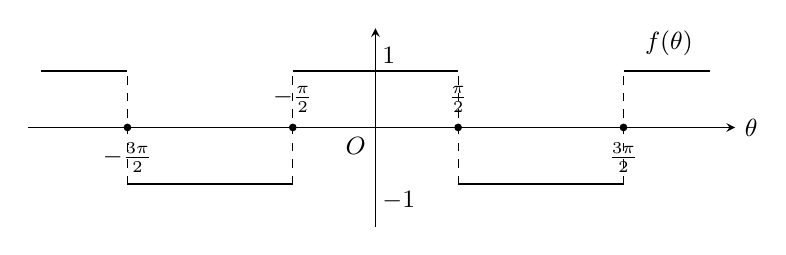
\begin{tikzpicture}[x=1.05cm,y=0.72cm,>=stealth,
 every node/.style={font=\small,fill=none,inner sep=0pt,outer sep=1.5pt}]
  \draw[->] (-4.2,0)--(4.35,0) node[right=2pt] {$\theta$};
  \draw[->] (0,-1.75)--(0,1.75);
  \draw[thick] (-4.05,1)--(-3.0,1);
  \draw[thick] (-3.0,-1)--(-1.0,-1);
  \draw[thick] (-1.0,1)--(1.0,1);
  \draw[thick] (1.0,-1)--(3.0,-1);
  \draw[thick] (3.0,1)--(4.05,1);
  \foreach \x in {-3,-1,1,3}{\draw[dashed] (\x,-1)--(\x,1); \fill (\x,0) circle (1.4pt);}
  \node[above right=1pt] at (0,1) {$1$};
  \node[below right=1pt] at (0,-1) {$-1$};
  \node[below=4pt] at (-3,0) {$-\frac{3\pi}{2}$};
  \node[above=4pt] at (-1,0) {$-\frac{\pi}{2}$};
  \node[above=4pt] at (1,0) {$\frac{\pi}{2}$};
  \node[below=4pt] at (3,0) {$\frac{3\pi}{2}$};
  \node[above=4pt] at (3.55,1) {$f(\theta)$};
  \node[below left=2pt] at (0,0) {$O$};
\end{tikzpicture}
\caption*{图2-4-1}
\end{figure}

（细心的读者会发现前式中我们既然写了 $|\theta|\le\dfrac{\pi}{2}$，所以在 $|\theta|=\dfrac{\pi}{2}$ 时两个式子矛盾了。我们这里是“故意”这样做的，因为今后我们会看到，若在“个别点”上改变函数值，有时并不影响讨论，详见第五章。但在目前的讨论中，确实应写为后式。）那么上式是不是仍表示一个函数？它既不是一个解析表达式，又不是可以“顺手”画出的曲线。这些事实迫使狄利克雷给出定义在区间 $A$ 上的函数的定义，即“有两个变量 $x$ 和 $y$，$x\in A$，而且对每个 $x$ 都有一个 $y$ 与之相应”，请读者注意，我们在定义中没有说什么“有确定的规律”或“有一定的方法”找出与 $x$ 对应的 $y$。因为什么叫“规律”，什么叫“方法”都是说不清的，是不是指某种“算法”？确有这样的函数，它是没有一定的算法来计算的，如此等等。这当然都是后来的人提出的问题（但决非无中生有的故作高深），狄利克雷本人不仅没有想到这一步，而且有时仍然说“完全任意的函数”都可以展开为傅里叶级数，其实他心里想的是适合狄利克雷条件的函数！由此可以想见传统的束缚和习惯的因素是多么有力！

傅里叶级数确实是一个产生重大数学成果的来源。狄利克雷自己考虑了具有第一类间断点的函数，如果有无穷多个间断点，那么可以考虑间断点的极限点。如果极限点只有有限多个还好说，有无穷多个又怎么办？是不是还应该考虑极限点的极限点呢？这样一来，人们所研究的函数范围就扩大到前人无法思议的地步。这时把函数定义为解析表达式或者某种图像都是无所助益的了。可是为什么要研究这种“病态”的函数？我们在第三章 §7 中将讲一些理由，而整个第四章实际上是围绕着这个问题来展开的：函数的类型越来越复杂，其反映大自然规律的深度越来越深，而到第六章，则对这些极丰富而又多样的对象给出了相当统一的框架，而丝毫不失严格性。到那里再来看初学者视为梦魇的 $\varepsilon-\delta$，就会感到还不过是雕虫小技，而有“会当凌绝顶，一览众山小”之慨！

那么，函数概念发展到这一步就“够用”了吗？问题的核心是某些自然现象所表现出的奇异性是古典的微积分（亦即所谓的古典分析）难以应对的。这里的情况和微积分的发展有些类似：人们在很长的时间里只能用一种不严格的、直观的方法，或者说是在没有充分根据的情况下沿用古典分析的概念与方法，然而总是得到了正确的结果。到了20世纪30年代，在许多数学物理问题中都出现了这种情况，使人们不能不认真地对待它们。然而幸运的是，到了20世纪50年代就系统地解决了这个矛盾，出现了所谓广义函数论（这是前苏联数学家的称呼，而西方数学界则称为分布理论）。我们在这里不可能详细地介绍它，而要在四、五两章中讲解其若干基本点。现在我们从一个最简单、而且谁都认为不可回避的问题开始。我们的讲法大体上相应于20世纪中没有掌握广义函数论的物理学家处理这类问题的方法，但随时指出其不足之处。但在本节最后，我们却要讲一个十分重要的定理，我们对它的处理将是严格的，而且证明的思想却很好地表现了广义函数的力量。

假设有一根棒，我们不妨设它是整个实数轴。如果从最左端算起直到 $x$ 点的这一段，其质量是 $m(x)$（当然我们不妨设 $m(x)$ 是有限的，因为总质量为 $\infty$ 的棒是很难设想的），我们来算一下，它在各点处的密度。为此，在棒上取 $(x,x+\Delta x)$ 一小段，其质量应该是
\[
\Delta m=m(x+\Delta x)-m(x),
\]
所以其平均密度是
\[
\frac{\Delta m}{\Delta x}=\frac{m(x+\Delta x)-m(x)}{\Delta x},
\]
而 $x$ 点的密度是一个函数
\[
\rho(x)=\frac{dm(x)}{dx}.
\]
只要 $m(x)$ 可求导，以上的作法就是合理的，又因 $m(x)$ 是从最左端 $x=-\infty$ 算起的，所以 $m(-\infty)=0$，因此又有
\[
m(x)=\int_{-\infty}^{x}\rho(x)\,dx,
\]
只要 $\rho(x)$ 是比较“规则”的，例如是连续的，而且这个积分又是收敛的，这个作法也是合理的。总之，在适当的“光滑性”（光滑一词就是指直到某阶导数均为连续）以及 $\rho(x)$ 的可积性条件下总有
\[
\rho(x)=\frac{dm(x)}{dx},
\qquad
m(x)=\int_{-\infty}^{x}\rho(x)\,dx. \tag{1}
\]

可是我们来看，若有一个单位质量的质点放在 $x=0$ 处，而棒的其它地方都没有质量，这时还有没有密度？(1)式是否成立？这个情况当然也是理想化的，但是很自然的。先计算 $m(x)$。若 $x<0$，则 $m(x)=0$；若 $x\ge0$，则 $m(x)=1$，所以 $m(x)$ 就是赫维赛德（O. Heaviside，1850--1925）函数：
\[
m(x)=H(x)=
\begin{cases}
1, & x\ge0,\\
0, & x<0.
\end{cases} \tag{2}
\]
读者会看到，若限于 $-\pi<\theta<\pi$，则上面我们讲的
\[
T(1,\theta)=f(\theta)=2\left[H(\cos\theta)-\frac12\right]
\]
\jiaokan{原文此处印作 $2[H(\theta)-\tfrac12]$。结合前文 $f(\theta)$ 在 $|\theta|<\pi/2$ 取 $1$、在 $\pi/2<|\theta|<\pi$ 取 $-1$，且下文继续讨论 $|\theta|=\pi/2$ 处的取值，显然应为 $H(\cos\theta)$。}
在那里我们说，在 $|\theta|=\dfrac{\pi}{2}$ 处，$f(\theta)$ 用哪个式子来表示并不重要，但现在却严格规定了 $H(0)=1$。这是因为在 $x=0$ 处有一个单位质量存在。赫维赛德是一个电气工程师，他研究一个电路，如果在某一瞬间 $x=0$（这里 $x$ 表示时间）把电路接通，输入一个单位电流，则在 $x\ge0$ 时，电流为1，$x<0$ 时，电流为0，他认为这种情况在研究电路理论中是最基本的。在某种意义下，这就是广义函数论的开始，时为1890年左右。

这种质量分布的密度是什么呢？现在我们暂把数学严格性的要求置诸脑后。如果 $x<0$，则只要 $\Delta x$ 充分小，仍有 $x+\Delta x<0$，因此
\[
\Delta m=m(x+\Delta x)-m(x)=0-0=0,
\]
$\Delta m/\Delta x=0$，其极限也为0。即当 $x<0$ 时，$\rho(x)=0$。若 $x>0$，则当 $\Delta x$ 充分小时，仍有 $x+\Delta x>0$，所以 $\Delta m=m(x+\Delta x)-m(x)=1-1=0$，我们仍有 $\rho(x)=0$。可是，注意，这里开始出问题了，如果我们把 $x$ 放在 $x=0$ 的“紧左边”，从而 $m(x)=0$，而若 $x+\Delta x$ 在 $x=0$ 的“紧右边”，则 $m(x+\Delta x)=1$，从而 $\Delta m/\Delta x=1/\Delta x$，而
\[
\rho(0)=\infty.
\]
大家立刻会看到，这已经不是数学语言了：什么叫紧左边，什么叫紧右边？无非是要把这个质点放在区间 $[x,x+\Delta x]$ 内，我们取极限时不只令 $\Delta x\to0$，而且也令 $x\to0$。这当然好办，我们只需取区间
\[
\left[-\frac{\Delta x}{2},\frac{\Delta x}{2}\right],\qquad \Delta x>0
\]
即可。可是这个极限是不存在的。习惯了数学思维的读者会问，怎么能够把不存在的东西叫密度呢？可是对物理学家，包括狄拉克（P. A. M. Dirac，量子物理学的大师）在内，却认为这是非常自然的，试想区间之长 $\Delta x$ 是一个无穷小，可是这个区间中的质量 $\Delta m=1$，二者一除不是无穷大又是什么呢？狄拉克当时的想法也就在这个水平上。如果伯克莱主教再世，他很可能会写一篇《不信神的物理学家》，并且说：狄拉克先生，您连量子力学那样稀奇古怪的东西都相信，凭什么不相信上帝呢？带着罪恶的灵魂怎么能进天国呢？难怪哲学家拉卡托斯（J. Lakatos）在《证明与反驳》一书中要再调侃一番了：牛顿等了两百多年，才有人出来拯救他的灵魂，进了数学的天堂，狄拉克要幸运得多，他还在世时，施瓦兹（L. Schwarz，有两个施瓦兹，这一位是法国数学家，另一位是 H. A. Schwarz，德国人，魏尔斯特拉斯的高足，我们每日每时都在用他的不等式。你不要忘了，我们每时每分都用的 $\varepsilon-\delta$ 并不是发表在什么 SCI 刊物上，而是见于他听自己的老师讲课所记的笔记中。为了区别，以后都用施瓦茨来表示德国人；而法国人都译为“施瓦兹”。——本书作者注。）就拯救了他的灵魂。狄拉克于1984年去世，可是施瓦兹在1950年就发表了《分布理论》（这个名词的来源很清楚了，我们讨论的不是一种质量分布吗？）一书，完全符合现代数学严格性要求，处理了狄拉克的理论。

这里有一个重要的争论：物理学家会说，难道狄拉克需要人来拯救他的灵魂吗？他已经在天国安息，当然天国里也会给施瓦兹留下位置。可是狄拉克一定会坐在更加紧靠上帝的椅子上。施瓦兹的“灵魂”的一部分，即施瓦兹核定理，不是狄拉克早已知道，并以自己的语言来陈述过？这可是你们数学家说的，请看冯·诺依曼（Von Neumann）《量子力学的数学基础》25--27页。数学家当然也可以反唇相讥：不妨再看一下爱因斯坦，难道不是黎曼给了爱因斯坦以灵魂吗？这可是爱因斯坦自己也承认的。这样的争论已经有多少年了，还会继续多少年？看来，数学与物理学是两种不同的文化，各有自己的方法与风格，然而都有共同的目标——探讨大自然的奥秘，而且携手并肩，结伴前进。

不论如何，我们得到了一个“函数”，狄拉克称之为 $\delta$ 函数，而且现在有公认的记号 $\delta(x)$：
\[
\delta(x)=
\begin{cases}
\infty, & x=0,\\
0, & x\ne0.
\end{cases}
\tag{3}
\]
但读者可以看出一个问题：如果我们在 $x=0$ 处放一个质量为2的质点，则一方面看，我们应得到 $2\delta(x)$，另一方面，我们又看到，会得到
\[
\frac{\Delta m}{\Delta x}=\frac{2}{\Delta x},
\]
仍是无穷大，归根结蒂：$2\infty=\infty$，因此仍会得到 $\delta(x)$。为了区别这些情况，我们在定义 $\delta$ 函数时还需要附加一个表示总质量为1的条件：
\[
\int_{-\infty}^{\infty}\delta(x)\,dx=1.
\tag{4}
\]
$\delta$ 函数即由(3)、(4)两式来“定义”。我们现在可以把这个“定义”中“不合法”的地方再重复一下：首先，一个函数应该对 $x$ 之每个值均有一个确定值与之对应，而 $\infty$ 肯定不能算是一个确定的值。其次，一个函数在某些点没有定义也是常有的事，这时定义其积分时常也是可以的，但按(3)式，$\delta(x)$ 的“积分”应该为0，而不应该是(4)式。

$\delta$ 函数最早是由赫维赛德在1894--1895年间定义的，1927年狄拉克在他关于量子力学的基本论文(1927年)提出以上的讲法，可以在狄拉克《量子力学原理》第二章 §15（P. A. M. Dirac, \textit{Principles of Quantum Mechanics}, 4th ed., Clarendon Press, 1958, 58--61页）中找到。在他的基本论文（\textit{The physical interpretation of the quantum dynamics}, Proc. of the Royal Soc. of London, A113, (1927)621--641）中，他说“当然，严格说来，$\delta(x)$ 并不是 $x$ 在本来意义下的函数，但是可以看作是某个函数序列的极限。完全同样，把它用于量子力学，对其几乎所有的需要，都不会得出不正确的结果”。

狄拉克在那本书和那篇论文中提出了两种解释 $\delta$ 函数的方法，一是利用对偶性（这是现代的语言，狄拉克那时是说用分部积分法），一是利用函数序列的极限。下面我们再加上一种利用测度的方法，则来自施瓦兹，其实也是对偶性之一例。我们将在第四章中讲解对偶性与函数序列的“极限”，现在我们先来不太严格地介绍测度方法，使读者有机会接触一点现代数学的思想和方法。

这本书里将不会一般地讨论测度理论，我们只直观地指出，测度是一个“集函数”。以一维情况为例，如果作一个分划
\[
-\infty<\cdots<a_1<\cdots<a_{n-1}<a_n<\cdots<+\infty,
\]
则可得一系列左闭右开的区间 $\sigma_n=[a_{n-1},a_n)$ 把实数轴 $\mathbf R$ 覆盖起来：$\mathbf R=\bigcup_{n=-\infty}^{\infty}\sigma_n$，对每个区间 $\sigma_n$，我们规定一个实数 $m(\sigma_n)$，使得
\[
m\!\left(\bigcup \sigma_i\right)=\sum_i m(\sigma_i).
\tag{5}
\]
这样的 $m$ 当然是一个“集函数”，即对集 $\sigma_n$ 确定了一个实数 $m(\sigma_n)$ 与之相应，测度的例子很多，通常的区间长度是一个测度。如上面所说的棒上的质量分布也是测度。这里有两点需要说明：首先我们是从区间 $\sigma_n$ 而不是更一般的集合开始，而且(5)式中的 $\bigcup$ 与和 $\sum$ 都不明确规定是有限并（有限和）还是可数并（可数和）。我们在这里虽然含糊其辞了，好在读者们在第四章会有机会读到准确的论述。其次，我们取 $\sigma_n$ 为左闭右开的而且彼此不相交，这却是重要的，因为我们要考虑集中在某一点的质量，如果该点在 $x=a_n$，则这个点的质量是算在 $[a_{n-1},a_n]$ 的质量内还是算在 $[a_n,a_{n+1}]$ 内呢？我们不能把一个质点的质量算两次，那会使棒的总质量产生疑义。总之，我们称适合(5)的 $m(\sigma)$ 叫做测度。有了测度就可以定义积分：设 $f(x)$ 充分光滑，而且在某有限区间 $[A,B]$ 之外恒为0，则可以定义 $f(x)$ 关于测度 $m(\sigma)$ 的积分为
\[
\int f(x)\,dm=\lim\sum_i f(\xi_i)m(\sigma_i).
\tag{6}
\]
这个积分称为黎曼—斯蒂尔切斯（Stieltjes）积分，它与黎曼积分的区别在于黎曼积分使用了一个特别简单的测度：$m(\sigma_n)=\{a_n-a_{n-1}\}$。$\delta$ 函数则相应于上面讲的有一个单位质量的质点位于 $x=0$ 处的测度。我们很容易计算这时的(6)式，设 $x_0=0$ 位于 $[a_j,a_{j+1})$ 内，则(6)式右方各项除了 $i=j$ 一项外全为0，从而只余下一项 $f(\xi_j)\cdot1$，$\xi_j\in[a_j,a_{j+1})$。由于我们假设了 $f(x)$ 充分光滑，故有
\[
\int f(x)\,dm=f(0).
\tag{7}
\]

这里我们必须在观念上有一个大转变：过去讲函数总是讲的可以在某一集合上逐点取值的“东西”（当然“逐点取值”有时可以马虎一点，在积分一章中我们还要回来讲怎样“马虎”）。现在，$\delta$ 函数则对应于一个测度，测度可不是逐点取值的东西，而是在某个集合 $\sigma_n$ 上有一个值。但是，它可以作用在一个充分光滑的函数 $f(x)$ 上，按(7)式起一种作用，即取出该函数（以后称为试验函数）在 $x=0$ 处的值来。凡是可以按某种线性的规律如(7)在一类试验函数上取值的对象，叫做一个线性泛函。一个普通的连续函数 $\varphi(x)$ 也可以在一类试验函数上取值，例如按下式
\[
(\varphi,f)=\int \varphi(x)f(x)\,dx
\tag{8}
\]
取值。如果 $\varphi(x)$ 有原函数 $\Phi(x)$，则(8)式还可以写为
\[
(\varphi,f)=\int f(x)\,d\Phi.
\]
所以，普通的连续函数也可以形成泛函。但是泛函不一定由普通连续函数生成，而也可以由例如测度生成。所以我们把这些线性泛函叫做广义函数，其实还可以由更加复杂的东西生成更复杂的广义函数，$\delta$ 函数只是最简单的一例，它按
\[
(\delta,f)=f(0)
\tag{9}
\]
生成一个由测度给出的广义函数，就是上文讲的在 $x=0$ 处有单位质量的质点生成的测度。

这样，我们看到测度可以认为是函数概念的推广，测度理论是一个很重要的数学分支，它特别是概率论的基础。我们将在第四章讨论一个特别有用的测度——勒贝格测度以及勒贝格积分。它是黎曼积分直接的推广。至于更一般的测度和积分（包括斯蒂尔切斯积分）我们都不讲了。我们只指出，它们都构成广义函数，而未在广义函数理论中把这一类划分出来专门讨论，因为那是太费力了。

再看如何用分部积分法来解释 $\delta$ 函数。和上面一样，取 $f(x)$ 为一试验函数，即定义在 $(-\infty,+\infty)$ 上的充分光滑而且在一有限区间 $[A,B]$ 外恒为0的函数。若 $\varphi(x)$ 在 $(-\infty,\infty)$ 上有连续的一阶导数，则有
\[
\int_{-\infty}^{\infty}\varphi(x)f'(x)\,dx
=\int_A^B\varphi(x)f'(x)\,dx
=\left.\varphi(x)f(x)\right|_A^B-\int_A^B\varphi'(x)f(x)\,dx
\]
\[
=-\int_A^B\varphi'(x)f(x)\,dx=-(\varphi',f).
\tag{10}
\]
这里我们利用了试验函数 $f(x)$ 充分光滑且在 $[A,B]$ 外恒为0，从而 $f(A)=f(B)=0$。(10)告诉我们，若 $\varphi'(x)$ 连续，则 $(\varphi,f')$ 可以化为 $\varphi'$ 作用在 $f$ 上形成的泛函（再改变符号），但是可能有这样的情况，即 $\varphi'(x)$ 不一定是一个好的函数，但 $(\varphi,f')$ 仍可以化为作用在 $f(x)$ 上所成的泛函（再改变符号）。这时，何妨把这个泛函看作是 $\varphi(x)$ 在某种广义意义下的导数？这是数学中推广某个概念的常用的方法：某个对象（如这 $\varphi(x)$）在某种条件下（这里是：$\varphi'(x)$ 连续）具有某种性质（这里是：在试验函数 $f(x)$ 上产生一个泛函如(8)式），而另一个对象在缺少该条件时也具有此种性质，我们就说这个另外的对象在缺少该条件时，广义地具有此种性质。我们来看一下“另一个对象”的例子：即赫维赛德函数(2)。它不是连续可微的，因为 $H(x)$ 在 $x=0$ 时甚至不连续，但若按(8)式将它作用到试验函数 $f(x)$ 之导数 $f'(x)$ 上，我们有
\[
\begin{aligned}
\int_{-\infty}^{\infty}H(x)f'(x)\,dx
&=\int_0^B H(x)f'(x)\,dx
 =\int_0^B f'(x)\,dx\\
&=\left.f(x)\right|_0^B
 =-f(0)=-(\delta,f).
\end{aligned}
\]
右方除了相差一个符号外即是(9)式，因此，我们说 $\delta$ 函数即 $H(x)$ 在广义函数意义下的导数：
\[
H'(x)=\delta(x).
\]
这就完全解释了赫维赛德的思想的合理内核。

我们再来回顾一下这里的作法。我们有两种对象，其一是试验函数 $f(x)$，它的集合是一个线性空间，而其元素都是性质很好的函数；我们这里规定 $f(x)$ 充分光滑，而且在某有限区间之外为0。另一类对象如 $\varphi(x)$，也形成了一个线性空间，例如对于 $\varphi_1(x),\varphi_2(x)$ 我们也可以研究 $c_1\varphi_1(x)+c_2\varphi_2(x)$ 等等。它的元素则可以不太“规矩”，例如赫维赛德函数在 $x=0$ 不连续。这些对象甚至可以是测度，根本不是逐点取值的函数。但是，它们可以像连续函数一样，在试验空间的函数上生成线性泛函，只不过生成的方式可以是(9)，而不一定是(8)。这个空间称为试验函数的对偶空间，这个名词也是由线性代数中借来的，而例如 $\int\varphi(x)f(x)\,dx=(\varphi,f)$ 就好像线性代数中两个向量的内积一样。$\varphi(x)$ 虽然不规则，例如不能求导，但是 $f(x)$ 则很规则可以求导，而且我们可以利用(10)式，把对 $\varphi(x)$ 求导这个困难问题转移到对 $f(x)$ 求导上去，这就是对偶性的妙用。分部积分法就可以看成是利用对偶性把“困难”由 $\varphi(x)$ 身上“转嫁”到 $f(x)$ 身上的方法。因此是一个很深刻的公式。

广义函数就是试验函数空间上的线性泛函，它是线性代数的思想与微积分的思想融合的产物。它使我们摆脱了函数必须在某一集合之各点上取值这个限制，使得许多分析运算可以很顺利地推广到原来不能应用的领域，帮助我们研究物理科学中许多有高度奇异性的对象。

下面我们再来解释狄拉克“$\delta(x)$ 可以看作是某个函数序列的极限”这句话。狄拉克是一个伟大的物理学家，他高度尊崇数学对物理学的重要性。他甚至认为数学美是选择在理论物理学中走哪一条路的最终判据。他说“方程之美比之其与实验结果的符合更重要”。当二者不甚符合时“不必太丧气，因为二者不符可能是由于某些较小的地方……而在理论的进步中迟早会弄清楚的”，但是他又不甚注意数学的严格性。他本是在英国布里斯托（Bristol）大学学电工的，后来（1923）才到剑桥圣约翰学院做研究生，转入了理论物理领域。1932年他当选为剑桥大学卢卡斯数学讲座教授（Lucasian Professor of Mathematics），这是当年牛顿担任过的教职。狄拉克在大学中学的主要是工科数学。后来，他这样回顾自己的经历：“我愿解释一下工程师的训练和工程教育对于我所起的作用……过去，我只对完全准确的方程有兴趣。然而我受到的工程训练教会了我要容忍近似，我能够看到有时近似的东西也包含了相当的美。……我想，如果不是有过这种工程训练，我后来作的那一类工作是不会成功的，……我在后来的工作中主要是继续使用了工程师的非严格的数学。我想，你们会发现我后来的著作中都用了非严格的数学”。在狄拉克看来，一是对数学美的追求，一是卓越的洞察力才是成功的保证。这是非常值得我们深思的。下面我们将先用完全严格的方法证明一个著名定理，再从 $\delta$ 函数的观点去重新看待它，作为对狄拉克的方法论的一点小小回顾，并就此结束我们对函数概念的讨论。

\medskip
\noindent\textbf{魏尔斯特拉斯定理}\quad 设 $f(x)$ 为某有限闭区间上的连续函数，则总可找到一串多项式 $P_n(x)$ 在此闭区间上一致收敛于 $f(x)$。

\noindent\textbf{证}\quad 设 $f(x)$ 是 $[\alpha,\beta]$ 上的连续函数，这里 $0<\alpha<\beta<1$。可以把 $f(x)$ 连续地拓展到 $(-\infty,\infty)$ 上，而且使它在 $[-A,A]$（$A>1$）外恒为0，这样一来 $f(x)$ 就是一个试验函数了（试验函数的“充分光滑性”本来就有相当的活动余地，这里我们只要求它是连续的。这一段话只与以下讨论 $\delta$ 函数有关，与本定理之证明无关）。

考虑积分
\[
I_n=\int_{-1}^1(1-u^2)^n\,du,
\tag{11}
\]
将它分成两部分，一部分是在 $|u|\le n^{-1/3}$ 上积分，另一部分是在 $n^{-1/3}\le |u|\le1$ 上积分，即
\[
I_n=K_n+L_n
=\int_{-n^{-1/3}}^{n^{-1/3}}(1-u^2)^n\,du
+\int_{n^{-1/3}\le |u|\le1}(1-u^2)^n\,du.
\]
当 $n\to\infty$ 时，$K_n$ 之积分区域缩为一点，但是它的贡献却是几乎 $I_n$ 的全部：
\[
\lim_{n\to\infty}L_n/I_n=0.
\]
证明如下：在 $L_n$ 中，被积函数之最大值在 $|u|=n^{-1/3}$ 时达到，所以
\[
L_n<2(1-n^{-2/3})^n,
\]
$I_n$ 之积分区域则包含了 $[-\frac12 n^{-1/3},\frac12 n^{-1/3}]$，所以
\[
I_n>\int_{-\frac12 n^{-1/3}}^{\frac12 n^{-1/3}}(1-u^2)^n\,du
>\left(1-\frac14n^{-2/3}\right)^n\cdot n^{-1/3},
\]
因此
\[
L_n/I_n<2n^{1/3}
\left[
\frac{1-n^{-2/3}}{1-\frac14n^{-2/3}}
\right]^n.
\]
但是
\[
\frac{1-n^{-2/3}}{1-\frac14n^{-2/3}}
=1-\frac{\frac34n^{-2/3}}{1-\frac14n^{-2/3}}
\le1-\frac34n^{-2/3}<e^{-\frac34n^{-2/3}}.
\]
这里我们用到了不等式 $e^x>1+x$（$x\ne0$），计算一下 $e^x-1-x$ 之最小值即可得此式。总之
\[
L_n/I_n<2n^{1/3}e^{-\frac34n^{1/3}}\to0.
\]

现在我们可以来构造 $P_n(x)$ 了，我们需要的 $P_n(x)$ 是一个 $2n$ 次多项式
\[
P_n(x)=\frac1{I_n}\int_0^1 f(y)[1-(y-x)^2]^n\,dy
=\frac1{I_n}\int_{-x}^{1-x}f(x+t)(1-t^2)^n\,dt.
\]
用上面的式子并用二项定理把 $[1-(y-x)^2]^n$ 展开，就知道 $P_n(x)$ 是 $x$ 的 $2n$ 次多项式。变换 $y=x+t$ 则给出第二个式子。因为 $\alpha\le x\le\beta$，故
\[
-x\le-\alpha<0<1-\beta\le1-x.
\]
取 $n$ 充分大，使 $n^{-1/3}<\min\{\alpha,1-\beta\}$，则
\[
-x<-n^{-1/3}<n^{-1/3}<1-x.
\]
这样，
\[
P_n(x)=\frac1{I_n}\int_{-x}^{-n^{-1/3}}
+\frac1{I_n}\int_{-n^{-1/3}}^{n^{-1/3}}
+\frac1{I_n}\int_{n^{-1/3}}^{1-x}
=J_1+J_2+J_3.
\]
\[
\begin{aligned}
|J_1|+|J_3|
&\le\frac1{I_n}
\left|\int_{-1}^{-n^{-1/3}}+\int_{n^{-1/3}}^1\right|
|f(x+t)|(1-t^2)^n\,dt\\
&\le\frac{M}{I_n}
\left|\int_{-1}^{-n^{-1/3}}+\int_{n^{-1/3}}^1\right|
(1-u^2)^n\,du
=ML_n/I_n\to0,\\[-1pt]
&\hspace{3em} M=\max|f(x)|.
\end{aligned}
\]
这里趋于0是对 $x$ 一致趋于0。对于 $J_2$ 则利用积分中值定理而有
\[
J_2=\frac1{I_n}\int_{-n^{-1/3}}^{n^{-1/3}}f(x+t)(1-t^2)^n\,dt
=f(x+\theta)\frac{K_n}{I_n},
\qquad |\theta|\le n^{-1/3},
\]
再利用 $f(x)$ 的一致连续性以及 $I_n=L_n+K_n$，即知对 $x$ 一致地有
\[
J_2\to f(x).
\]
定理证毕。

魏尔斯特拉斯定理有许多发展。例如设 $f(x_1,\cdots,x_n)$ 为连续函数，而且对每个变量 $x_i$ 都有周期 $2\pi$，则 $f(x_1,\cdots,x_n)$ 一定可以用三角多项式
\[
\sum a_{k_1,\cdots,k_n}e^{\sqrt{-1}(k_1x_1+\cdots+k_nx_n)},
\qquad |k_1|,\cdots,|k_n|\le N
\]
去一致逼近。

现在我们从 $\delta$ 函数的观点来看这个证明。我们很容易想到 $I_n\to0$，因为计算这个积分并不难。所以 $\dfrac1{I_n}(1-u^2)^n$，当 $n$ 越变越大时，图形大抵如图2-4-2；当 $u\ne0$ 时，总有
\[
\lim_{n\to\infty}\frac1{I_n}(1-u^2)^n=0,
\]
但当 $u=0$ 时，
\[
\lim_{n\to\infty}\frac1{I_n}(1-u^2)^n=\infty,
\]
同时恒有
\[
\frac1{I_n}\int_{-1}^1(1-u^2)^n\,du=1,
\]
所以 $\dfrac1{I_n}(1-u^2)^n$ 之“极限”就是 $\delta$ 函数，而我们上面证明的定理其实就是说

\begin{figure}[htbp]
\centering
\begin{tikzpicture}[x=2.2cm,y=0.55cm,>=stealth]
  \draw[->] (-1.22,0)--(1.30,0) node[right=2pt] {$u$};
  \draw[->] (0,-0.18)--(0,7.1);
  \draw (-1,0.08)--(-1,-0.08) node[below=2pt] {$-1$};
  \draw (1,0.08)--(1,-0.08) node[below=2pt] {$1$};
  \node[below left=1pt] at (0,0) {$O$};
  \draw[thick,domain=-1:1,samples=160,smooth,variable=\u]
    plot ({\u},{0.75*(1-\u*\u)});
  \draw[thick,domain=-1:1,samples=160,smooth,variable=\u]
    plot ({\u},{1.55*(1-\u*\u)^3});
  \draw[dashed,thick,domain=-1:1,samples=180,smooth,variable=\u]
    plot ({\u},{4.7*(1-\u*\u)^12});
  \node[anchor=west] at (0.10,5.55) {$\dfrac{(1-u^2)^n}{I_n}$};
\end{tikzpicture}
\caption*{图2-4-2}
\end{figure}

\[
\lim_{n\to\infty}\int_{-1}^1\frac1{I_n}(1-t^2)^n f(t+x)\,dt
=\int\delta(t)f(t+x)\,dt=f(x).
\]
这就是狄拉克所说的用 $\delta(x)$“可以看作是某个函数序列的极限”的意思。但是，上面的讲法总是不严格的，因为只看
\[
\lim_{n\to\infty}\frac1{I_n}(1-u^2)^n=\infty\quad(u=0\text{ 时})
\]
以及
\[
\lim_{n\to\infty}(1-u^2)^n=0\quad(u\ne0\text{ 时}),
\]
不能就说函数极限就是 $\delta$ 函数
\[
\delta(u)=
\begin{cases}
\infty, & u=0,\\
0, & u\ne0.
\end{cases}
\]
再则，我们不能随意地在积分号下取极限，所以我们又只好说是一种“广义的”极限过程。我们称它是“弱极限”。但是应该说明，“弱极限”是一个很严肃的数学概念，读者以后有很多机会遇见它。

上面讲的函数序列，通常称为 $\delta$ 型序列，它在物理学中是很常见的。其中有一些是如上所示的“钟形曲线”，而有一些则完全令人联想不到这种图形，而表现出的剧烈的振荡特性。关于广义函数，包括这里讲的 $\delta$ 型序列，四、五两章中将比较详细地介绍。
